%%%% CAPÍTULO 3 - MATERIAL E MÉTODOS (PODE SER OUTRO TÍTULO DE ACORDO COM O TRABALHO REALIZADO)

\chapter{Materiais e Métodos}
\label{cap:materialemetodos}


%A ênfase deste capítulo está em reportar o que e como será feito para alcançar o objetivo do trabalho. Este capítulo pode ser subdividido, inicialmente, em duas seções, sendo uma para os materiais e outra para os métodos.
%
\section{Materiais}\label{sec:materiais}
%
%Materiais são as ferramentas, as tecnologias, os ambientes de desenvolvimento e outros que são utilizados para realizar as atividades desde a definição dos requisitos à implantação do sistema. Exemplos de materiais: linguagens de programação e de modelagem, banco de dados e seus gerenciadores, editores para análise e modelagem, ambiente e plataforma de desenvolvimento.
%
%Cada um dos materiais pode ter uma subseção própria ou serem descritos em uma mesma seção. De qualquer forma, essa seção não precisa ser muito extensa, deve abranger apenas um conhecimento básico sobre cada um dos materiais e o que é mais relevante ou utilizado para o trabalho proposto. De maneira geral, não há necessidade de incluir informações históricas sobre os materiais. Centrar-se nos conceitos e particularidades mais relevantes para o trabalho. Exceto se necessário para o entendimento do objeto do trabalho ou considerado relevante para o tipo de pesquisa.
%

As ferramentas de desenvolvimento do navegador, também conhecidas como \textit{DevTools}, são conjuntos de ferramentas incorporadas nos navegadores da web, como Google Chrome e Mozilla Firefox. Essas ferramentas permitem que os desenvolvedores da web inspecionem e depurem o código-fonte da página, além de analisar o desempenho, uso de memória de seus aplicativos da web, entre outros recursos \cite{apple}. Durante o desenvolvimento deste trabalho foram utilizadas as ferramentas listadas abaixo.

\subsection{Chrome DevTools}
O Chrome DevTools, Figura \ref{fig:chrome-devtools}, representam um conjunto abrangente de ferramentas integradas ao navegador Google Chrome, essenciais para o desenvolvimento e depuração de aplicações web. Com ele é possível inspecionar o DOM, analisar o desempenho da página, depurar JavaScript, simular diferentes dispositivos, entre outros recursos. \cite{chrome}.
\begin{figure}[!htb]
    \centering
    \caption{Chrome Devtools}
    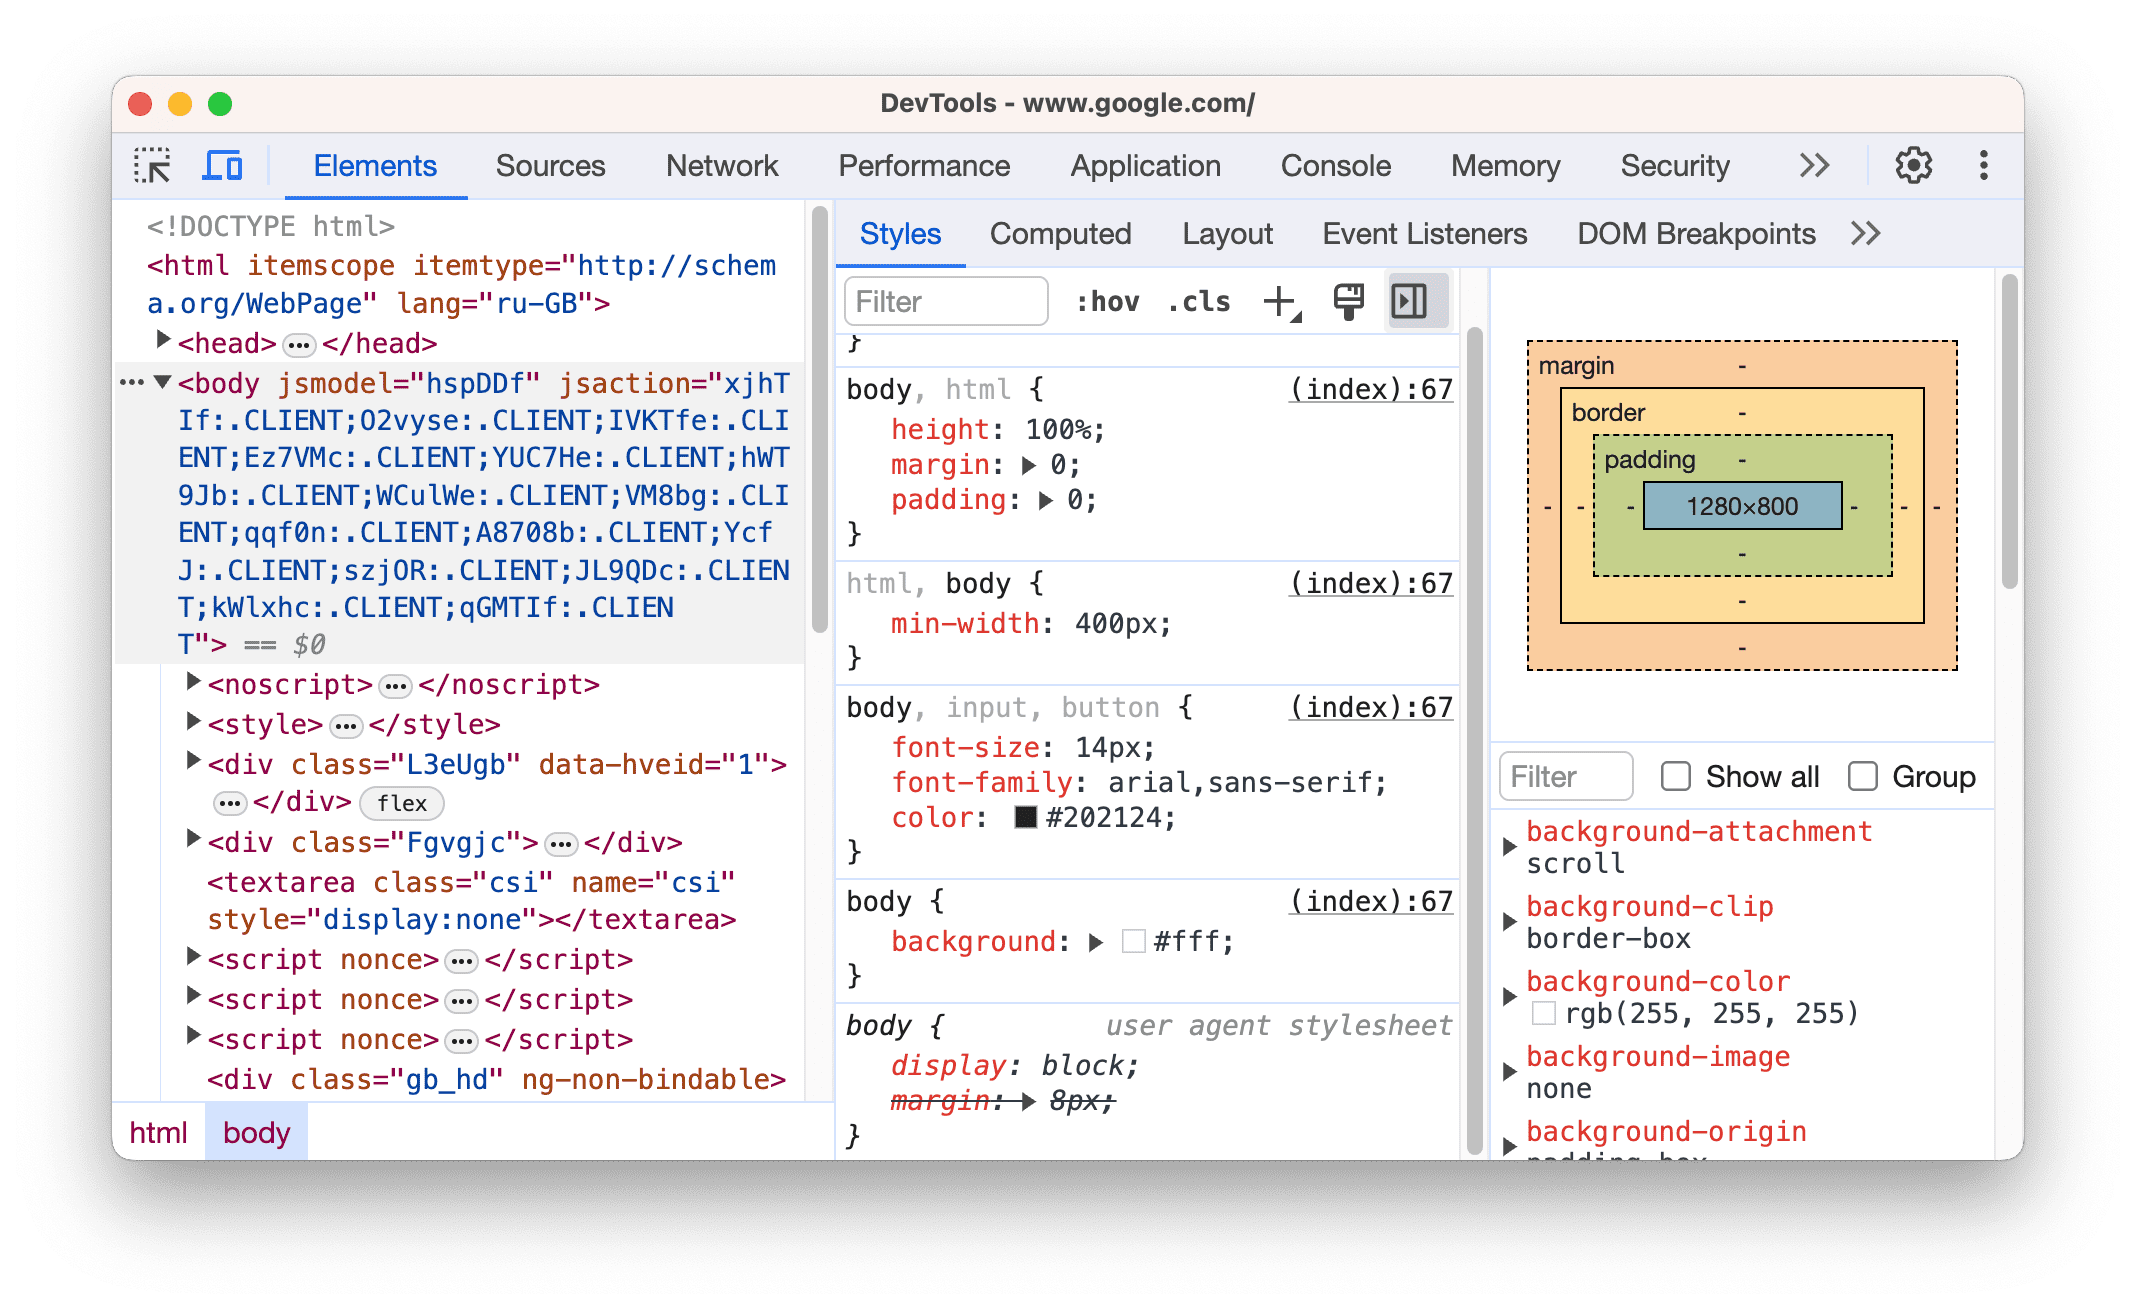
\includegraphics[width=0.65 \linewidth]{../figuras/chrome-devtools.png}\\
    {\footnotesize Fonte: Chrome for Developers}
    \label{fig:chrome-devtools}
\end{figure}
\newpage

\subsection{Firefox Developer Tools}
O Firefox Developer Tools, ilustrado na Figura \ref{fig:firefox}, oferece uma alternativa robusta aos Chrome DevTools, com um foco em privacidade e personalização. Essas ferramentas proporcionam um ambiente de desenvolvimento completo, permitindo a inspeção de elementos, a análise de redes, o depurador de JavaScript, a visualização de estilos CSS e a otimização do desempenho. Além disso, o Firefox Developer Tools se integra perfeitamente com outras ferramentas do ecossistema Mozilla, como o editor de código Visual Studio Code, facilitando o fluxo de trabalho dos desenvolvedores \cite{firefox}.
\begin{figure}[!htb]
    \centering
    \caption{Firefox Developer Tools}
    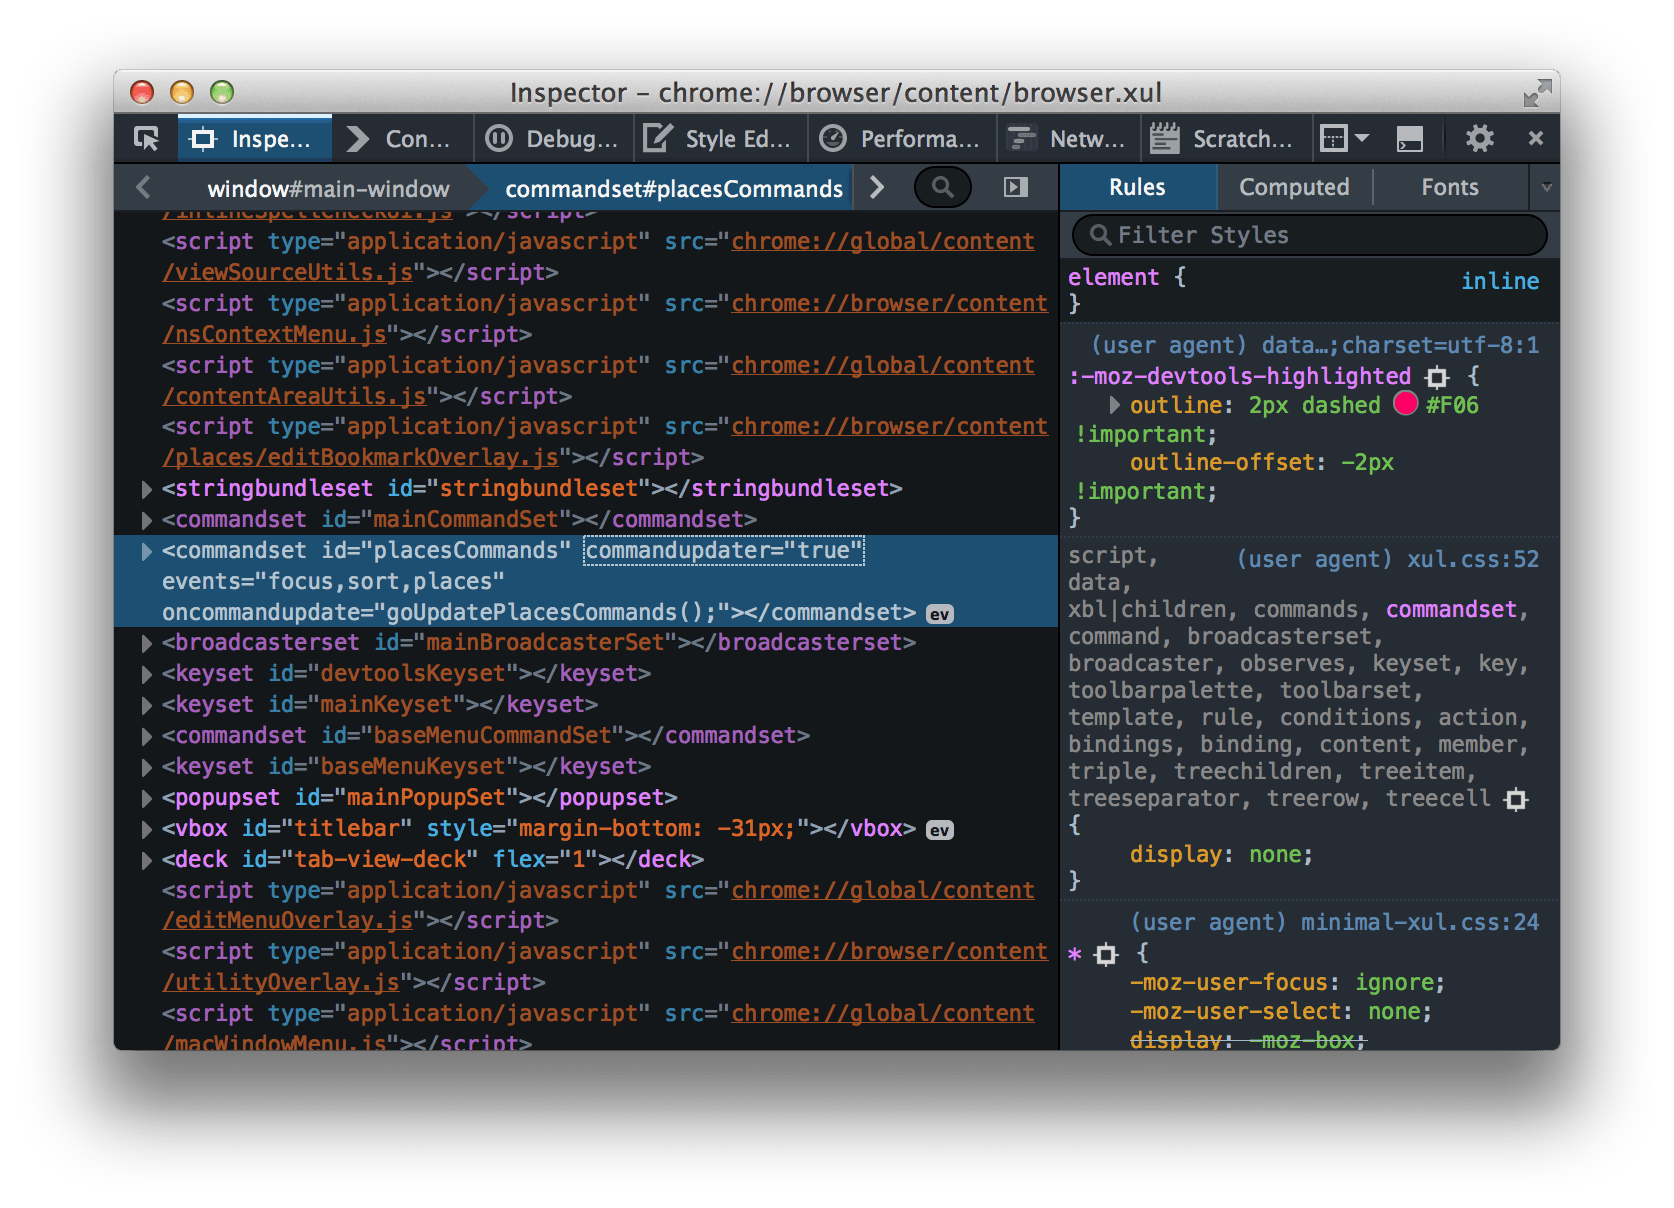
\includegraphics[width=0.8\linewidth]{../figuras/firefox.png}\\
    {\footnotesize Fonte: Firefox Source Tree Documentation}
    \label{fig:firefox}
\end{figure}

\subsection{Edge DevTools}
Os Edge DevTools, ilustrado na Figura \ref{fig:edge}, incorporados ao navegador Microsoft Edge, oferecem uma experiência de desenvolvimento moderna e eficiente. Com uma interface visualmente atraente e funcionalidades similares aos Chrome DevTools, os Edge DevTools permitem inspecionar elementos, depurar JavaScript, analisar o desempenho da página e simular diferentes dispositivos. A integração com o Microsoft Visual Studio Code e outras ferramentas do ecossistema Microsoft torna os Edge DevTools uma opção atraente para desenvolvedores que utilizam a plataforma Windows\cite{edge}.

\begin{figure}[!htb]
    \centering
    \caption{Edge DevTools}
    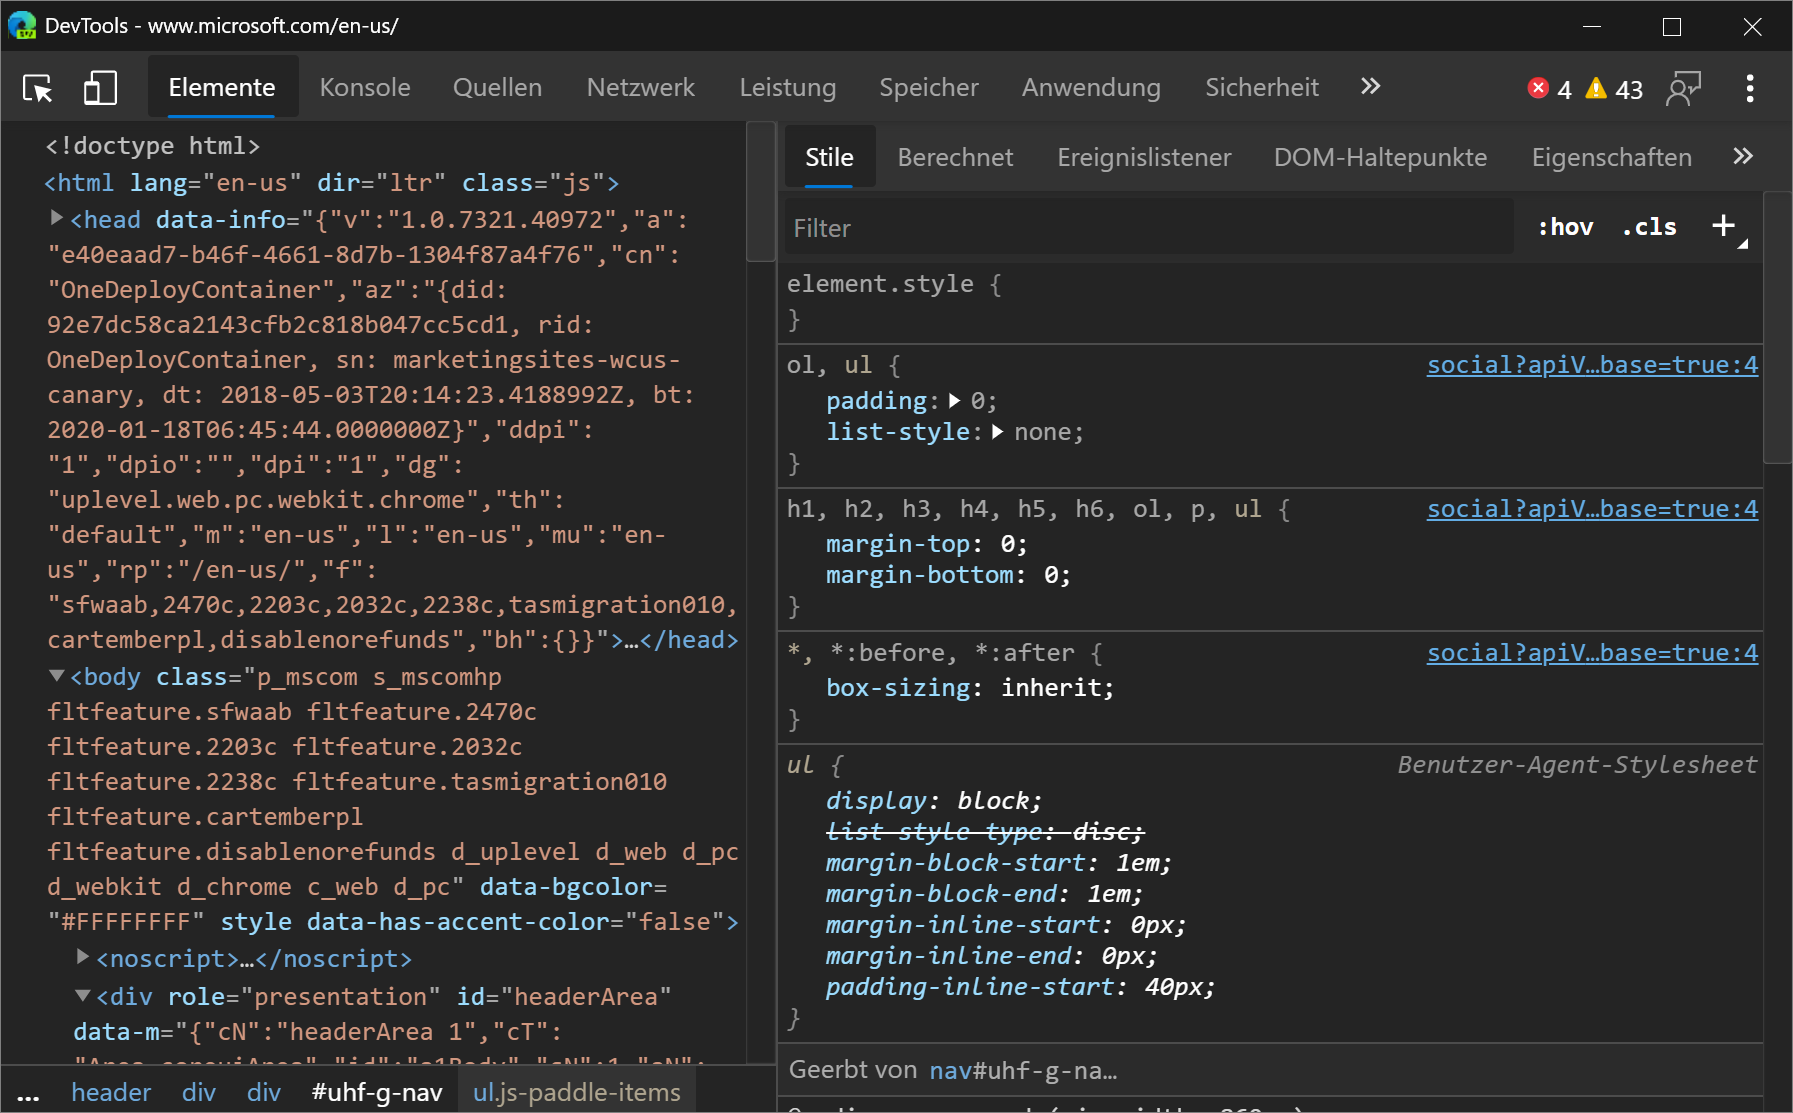
\includegraphics[width=0.8\linewidth]{../figuras/edge.png}\\
    {\footnotesize Fonte: Microsoft Learn}
    \label{fig:edge}
\end{figure}

\subsection{Safari Web Inspector}
O Safari Web Inspector, ilustrado na Figura \ref{fig:safari}, é a ferramenta de desenvolvimento integrada ao navegador Apple Safari, projetada para oferecer uma experiência de depuração e desenvolvimento de alta qualidade. Com um foco em desempenho e usabilidade, o Web Inspector permite inspecionar elementos, depurar JavaScript, analisar o desempenho da página e simular diferentes dispositivos\cite{apple}.
\begin{figure}[!htb]
    \centering
    \caption{Safari Web Inspector}
    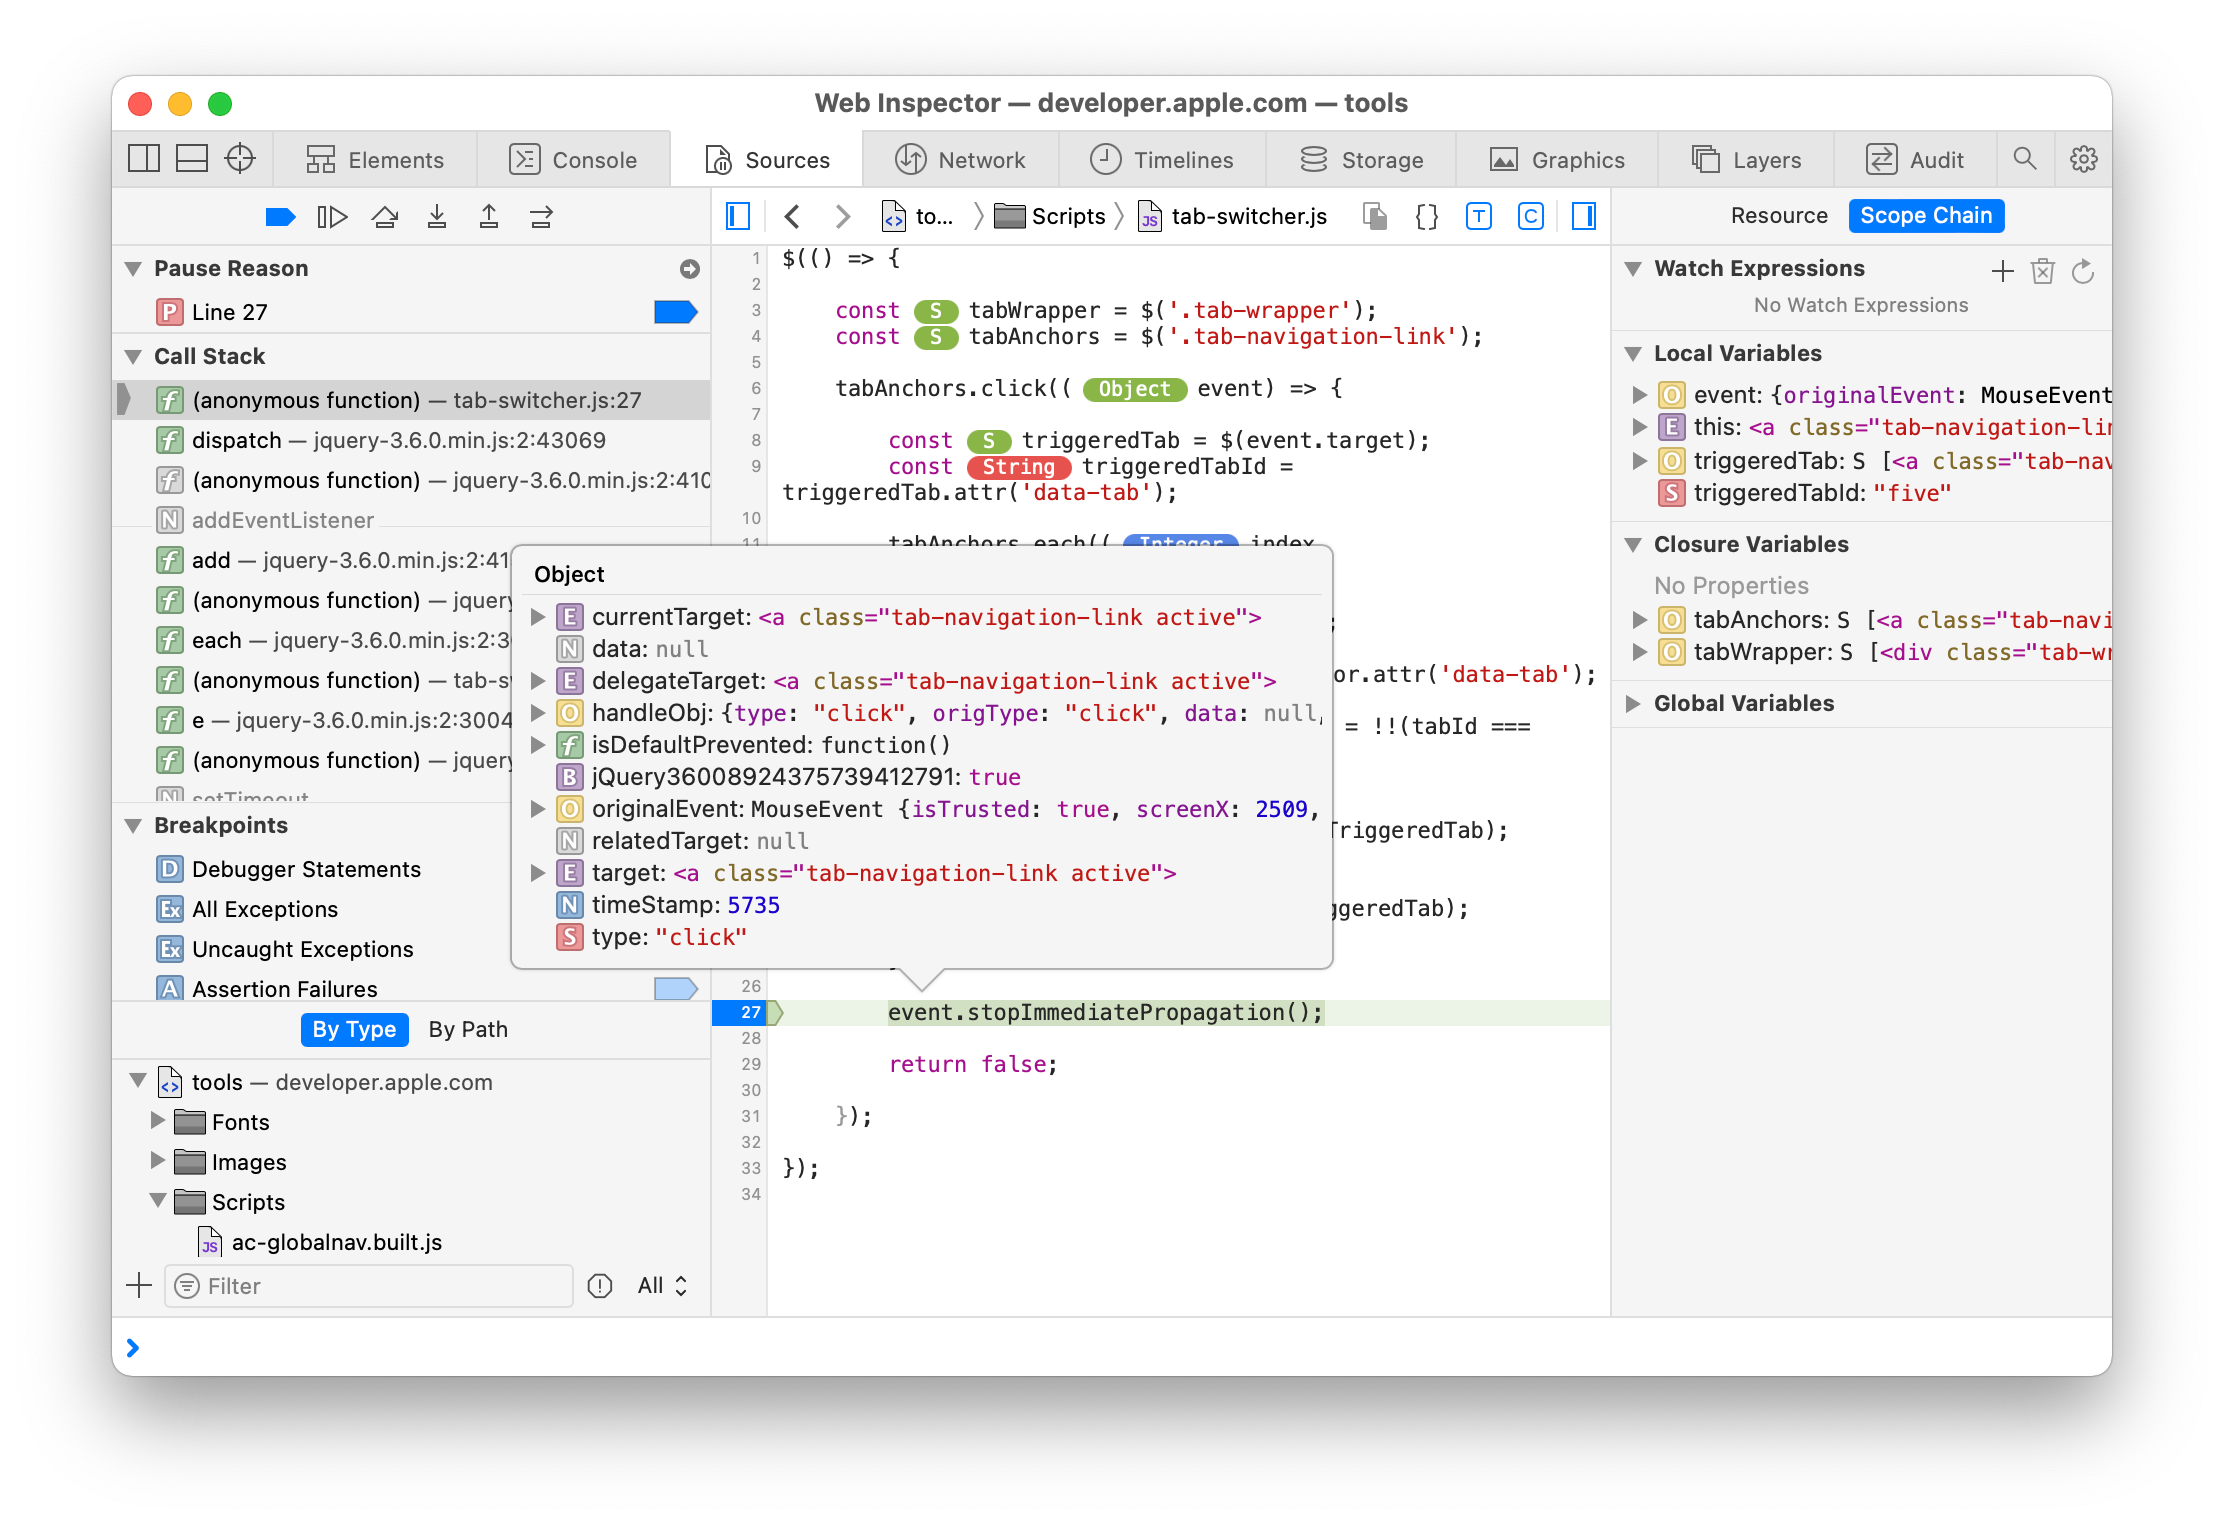
\includegraphics[width=0.8\linewidth]{../figuras/safari.png}\\
    {\footnotesize Fonte: Apple Developer Documentation}
    \label{fig:safari}
\end{figure}




\section{Métodos}\label{sec:metodo}
%
%Os métodos definem, de certa maneira, um plano geral do trabalho, com as principais atividades realizadas durante seu processo de desenvolvimento. São apenas as atividades, o que será feito e o que se espera obter com as mesmas. O que é obtido com a realização dessas atividades está no \autoref{cap:resultados}. 
%
%Os métodos são, basicamente, uma sequência de atividades realizadas para definir o sistema, modelar o problema e a solução, implementar a solução, testar e implantar essa solução. Essas atividades devem enfatizar a forma de uso dos materiais de acordo com o referencial teórico e como foi procedido no sentido de alcançar os objetivos do trabalho.
%Os métodos incluem os procedimentos utilizados para se alcançar o objetivo do trabalho. Assim, ele abrange o ciclo de vida do sistema, da identificação do problema à implantação da solução. A identificação pode incluir a definição dos requisitos por parte do usuário e/ou cliente definindo a proposta do sistema. A implantação pode incluir a forma de gerar os instaladores, os recursos e forma de instalação do sistema, a forma de manutenção e de descontinuidade do sistema.
%
%A definição das atividades, passos, ou procedimentos que compõem os métodos podem (ou mesmo deve) estarem baseados em autores. Esses autores, normalmente, estão relacionados à engenharia de software.
%
%O tempo verbal a ser utilizado na descrição dos métodos é o passado, considerando que trata-se de métodos que foram aplicados para a obtenção dos resultados a serem apresentados.

Para o desenvolvimento deste trabalho optou-se por uma abordagem de análise exploratória. Este método se mostra especialmente adequada para este tema. Este método permite um exame detalhado e flexível do tema, proporcionando analises valiosas sobre as funcionalidades e características das ferramentas investigadas, bem como suas aplicações práticas no contexto do desenvolvimento web.

O campo é caracterizado por um rápido avanço tecnológico e pela ampla diversidade de soluções disponíveis. Assim, uma análise exploratória permite identificar padrões, relações e tendências que não seriam facilmente percebidos por meio de abordagens mais restritivas ou estruturadas.

\subsection{Analise exploratória}
A análise exploratória é uma metodologia qualitativa que busca compreender fenômenos, identificar tendências e levantar hipóteses a partir de dados ou informações iniciais \cite{analise-exploratoria}. Em contraste com métodos estruturados, que partem de hipóteses previamente definidas, a análise exploratória permite maior flexibilidade e adaptação durante o processo, sendo amplamente utilizada em pesquisas iniciais ou contextos pouco conhecidos.

No contexto deste estudo, a análise exploratória se justifica por permitir uma investigação aberta das ferramentas de desenvolvimento web, explorando desde as funcionalidades nativas até extensões e práticas comuns entre desenvolvedores. Com isso, essa metodologia será utilizada para:

\begin{itemize}
    \item \textbf{Analisar as características das ferramentas}: comparar as funcionalidades, linguagens suportadas, comunidades e ecossistemas de cada ferramenta.
    \item \textbf{Identificar tendências}: observar a evolução das ferramentas ao longo do tempo, a emergência de novas tecnologias e a obsolescência de outras
    \item \textbf{Avaliar a percepção dos desenvolvedores}: por meio de pesquisas, compreender as preferências, necessidades e desafios dos desenvolvedores na escolha de ferramentas.
\end{itemize}

A aplicação dessa metodologia é realizada em etapas sequenciais, que envolvem desde a coleta de dados até a interpretação dos resultados obtidos.
